% Sune
%#############
% Hvad er copatterns?
% Hvorfor giver copatterns mening, isoleret set?
% Hvor kommer copatterns fra? (Hagino, Abel og venner)
% Definition ved observation (eliminationsregler)
% Eksempler

% Ny viden: Copatterns
%#############

\section{Copatterns}
\label{sec:copatterns}
In functional programming, inductive data is commonly defined by \emph{constructors} in an
elegant and simple fashion. The data can be analyzed and manipulated using
pattern matching, which follows nicely from the finite nature of inductive
data. Due to its possible infinity, it is appealing to define coinductive data by
\emph{observations}, rather than constructors. This means that one should distingush
between finite and infinite data. The idea of describing infinite data by their
observations was pioneered by Hagino  in his SymML language \,\citep{Hagino89}, where the programmer could define coinductive types
by their \emph{destructors} or \emph{observations}. 

This duality between inductive and coinductive types is discussed in
detail in Section~\ref{sec:coinductive-types}. As a part of this project we have
introduced a new syntax for defining coinductive types by their
observations. This new coinductive record, or just \emph{corecord}, syntax is described in
Appendix~\ref{app:record-types-observ}. An example of this syntax can be seen in Figure~\ref{fig:stream}.

% In other words\todo{We have
%   to be precise here. }, inductive
% types should be defined by their \emph{introduction rules}, and coinductive types by
% their \emph{elimination rules}.

\begin{figure}[h]
\begin{lstlisting}[mathescape]
corecord Stream a where
  head : a
  tail : Stream a 
  constructor MkStream
\end{lstlisting}
\caption{An infinite stream defined by observations.}
\label{fig:stream}
\end{figure}

The syntax for \texttt{corecord} definitions presented in
Figure~\ref{fig:stream} defines a coinductive type by observations, as oppose to
by constructors. On a \texttt{Stream}, two observations can be made:
\texttt{head} and \texttt{tail}. The former provides us with the first element
of the stream, while the latter gives us with the rest of the infinite stream,
upon which another element can be observed with \texttt{head}. 

\emph{Destructor copatterns}, or simply
\emph{copatterns}\,\citep{Abel13Copatterns}, provide a way of defining functions
on coinductive data in terms of observations. Like pattern matching allows us to
define functions on inductive data by analyzing the structure of the input,
copatterns enable us to perform experiments on functions with a result of
coinductive type.

The \texttt{Stream} defined by observations can be used to define a function
\texttt{nats}, a list of all natural numbers, using copatterns, as shown in
Figure~\ref{fig:nats_copatterns}.


\begin{figure}[h]
\begin{lstlisting}[mathescape]
nats : Stream Nat
head nats = Z
tail nats = map S nats
\end{lstlisting}
\caption{A definition of \texttt{nats} using copatterns.}
\label{fig:nats_copatterns}
\end{figure}

Because the result type of \texttt{nats} is defined by observations, we can use
copatterns to define the outcomes of our observations. The intuition is that the
first element of \texttt{nats} is zero (\texttt{Z}), and the rest of the natural
numbers are all the natural numbers incremented by one (\texttt{map S
  nats}). Initially, the \texttt{head} observation will therefore return
\texttt{Z}. Making a \texttt{tail} observation results in a new stream where all
the elements of \texttt{nats} are incremented by one (using the \texttt{S}
constructor for natural numbers). Consequently, the outcome of making a
subsequent \texttt{head} observation is \texttt{S Z}. As we can increment a
natural number infinitely many times, we can also make infinitely many
\texttt{tail} observations, where the result of a \texttt{head} observation will
be incremented for each \texttt{tail} observation. 

Syntactically, projection happens on the outside of definitions when we use
copatterns, as opposed to pattern matching, where projection on parameters
happens inside of definitions. As an example, consider the definition of
\texttt{map} in Figure~\ref{fig:map_copatterns}.

\begin{figure}[h]
\begin{lstlisting}[mathescape]
map : (a -> b) -> Stream a -> Stream b
head (map f s) = f (head s)
tail (map f s) = map f (tail s)
\end{lstlisting}
\caption{The \texttt{map} function defined with copatterns.}
\label{fig:map_copatterns}
\end{figure}

For \texttt{map}, it is clear that the observations are applied on the entire
definition \texttt{map f s}. Projections on the entire definition make sense
because \texttt{map f s} has the coinductive type \texttt{Stream b}, which can
be the subject of observations. In this sense, copatterns can be said to be dual
to pattern matching in the same way that coinductive data is dual to inductive
data. With pattern matching, we can analyze how data has been constructed, and
with copatterns we can define the outcome of observations. Where pattern
matching is a way of processing input, copatterns provide the means for
describing output. 

\subsection{The Anatomy of Copatterns}
Definitions using copatterns are made of multiple different parts. To be better
communicate about copatterns we establish the following names, also denoted in
Figure~\ref{fig:copatterns_anatomy}:

\newcommand{\itemEmph}[1]{\item \emph{#1}:}

\begin{itemize}
\itemEmph{Observation pattern} An observation, or projection, on the
  left-hand side of a definition.
\itemEmph{Pattern} A function name and a possible list of argument patterns.
\itemEmph{Argument pattern} A pattern for an argument to a function. Can be a
variable pattern, a constructor pattern or a wild card pattern.
\itemEmph{Copattern} An observation pattern performed on a pattern.
\itemEmph{Nested copattern} A copattern under an observation pattern.
\itemEmph{Pattern clause} An entire clause, both left- and right-hand side,
without copatterns.
\itemEmph{Copattern clause} As a pattern clause, but with an observation pattern.
\end{itemize}

\begin{figure}[H]
\centering
  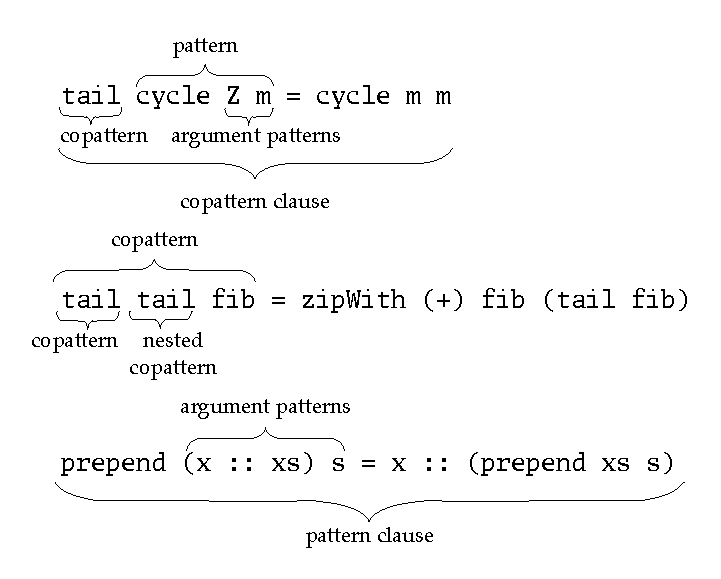
\includegraphics[scale=1]{figures/copattern_anatomy}
  \caption{The anatomy of copatterns.}
  \label{fig:copatterns_anatomy}
\end{figure}

\subsection{Existing Implementations of Copatterns}
Copatterns already exist in programming languages, for example in
Agda\,\cite{Norell:thesis}. Here, definitions for coinductive types are quite
interesting. A coinductive type is defined as a record type with a
\texttt{coinductive} flag, an example of which can be seen in
Figure~\ref{fig:agda_stream}. Observations are defined as fields of the record
type.

\begin{figure}[h]
\begin{lstlisting}[mathescape]
record Stream (A : Set) : Set where
  coinductive
  field
    head : A
    tail : Stream A
open Stream
\end{lstlisting}
\caption{\texttt{Stream} definition in Agda.}
\label{fig:agda_stream}
\end{figure}

Definitions with copatterns are almost identical to what has already been
discussed. A simple example \texttt{repeat} in Figure~\ref{fig:agda_repeat}. 

\begin{figure}[h]
\begin{lstlisting}[mathescape]
repeat : {A : Set} -> A -> Stream A
head (repeat a) = a
tail (repeat a) = repeat a 
\end{lstlisting}
\caption{A corecursive \texttt{repeat} function in Agda.}
\label{fig:agda_repeat}
\end{figure}

In Section\,\ref{sec:motivation_copatterns} we discuss the motivation behind the
use of copatterns. Later, in Chapter\,\ref{sec:adding_copatterns}, we describe
how we have added a syntax for copatterns to the programming language Idris. The
syntax we have added to Idris includes a prefix character, \texttt{\&}, on the
observation patterns, as pictured
Figure~\ref{fig:map_copat_syntax}. In the remaining report we will use this
syntax for copattern definitions.

\begin{figure}[h]
\begin{lstlisting}[mathescape]
map : (a -> b) -> Stream a -> Stream b
&head (map f s) = f (head s)
&tail (map f s) = map f (tail s)
\end{lstlisting}
\caption{The \texttt{map} function defined with copatterns using the syntax
  described in Chapter~\ref{sec:adding_copatterns}.}
\label{fig:map_copat_syntax}
\end{figure}

%%% Local Variables: 
%%% mode: latex
%%% TeX-master: "../../copatterns-thesis"
%%% End: 
